\documentclass{article}
\usepackage{neurips_2023}

\usepackage[utf8]{inputenc} % allow utf-8 input
\usepackage[T1]{fontenc}    % use 8-bit T1 fonts
\usepackage{hyperref}       % hyperlinks
\usepackage{url}            % simple URL typesetting
\usepackage{booktabs}       % professional-quality tables
\usepackage{amsfonts}       % blackboard math symbols
\usepackage{nicefrac}       % compact symbols for 1/2, etc.
\usepackage{microtype}      % microtypography
\usepackage{xcolor}         % colors
\usepackage{graphicx}       % images & graphics

\title{Man, I Just Love Writing Research Papers}
\author{%
  Jacob Badolato \\
  University of Texas at Austin \\
  \texttt{jacobbadolato@utexas.edu} \\
  \And
  Andrew McGehee \\
  University of Texas at Austin \\
  \texttt{andrewmcgehee@utexas.edu} \\
}

\begin{document}

\maketitle

\begin{abstract}
	State of the art language models have been shown to perform well across a broad spectrum of language modeling tasks like natural language inference (NLI), question answering (QA), and next token generation tasks as seen in applications like ChatGPT \cite{naveed2023comprehensive}. However, it is still quite simple to find examples that confuse language models and cause significant degradation in performance metrics. In this work, we propose one such set of "tricky" examples. We analyze the performance of the ELECTRA-SMALL model \cite{clark2020electra} on the NLI task \cite{bowman-etal-2015-large} across three subsets of tricky examples: sarcasm, grammatically incorrect dialect, and idiomatic speech. We show that the model struggles to accurately classify such examples. While the model achieves a strong 85.8\% accuracy on the Stanford NLI (SNLI) dataset \cite{bowman-etal-2015-large}, it is only able to achieve 50.9\% accuracy on the holdout portion of our curated tricky dataset. We also show that simply fine tuning the model on a small training portion of these examples improves the models ability to accurately classify new tricky examples while incurring almost no additional loss on the original SNLI dataset. Hence, we provide some evidence that providing higher quality, more diverse examples of real, albeit complex language patterns in training data can improve a model's ability to generalize across tricky examples.
\end{abstract}

\section{Introduction}
Models like GPT 3 \cite{brown2020language}, GPT 3.5 Turbo, and \cite{openai2023gpt4} GPT 4 have left the world speechless at the awe-inspiring
capabilities of large language models (LLMs). In contrast, LLM failures like those in the early versions of Bing + ChatGPT
have served as comedic inspiration for memes as well as the inspiration of nightmares for Microsoft stakeholders. This
raises the question: given the strong results of LLMs in some domains, which problem classes cause LLMs to experience
performance degradations? This work begins to explore this question.

Drawing inspiration from some of the well-known LLM failures mentioned earlier, we devised a set of "tricky" examples to
test LLMs against, and we observed their behavior. These tricky examples are all examples of real language patterns that
humans can decipher with relative ease. The examples are subdivided into three groups:  sarcasm, grammatically incorrect
dialect, and idiomatic speech. We provide examples from each of these groups in a later section.
A criticism the reader may levy against the use of sarcasm in text is that the notions of tone,
body language, rate of speech, inflection, etc. aren't signals which are included in the text. The authors encourage those
with such criticisms to consider times where they have been able to decipher sarcasm in text messages without any additional
context. While the authors acknowledge the limitation that even humans cannot perfectly decipher sarcasm via text alone,
it is certainly an achievable task and therefore still within the scope of our research question.

We interrogate this question by training an instance of the ELECTRA-SMALL model. Despite its proven capabilities on other datasets,
the model struggles with our tricky examples. Sarcasm, dialect, and idioms are often context dependent, non-literal, and
difficult to parse grammatically. The authors expected when devising these examples that the model would struggle with these
examples for the following reason:  the "default mode" of speech in most language training data is literal, mostly grammatically
correct, and directly interpretable with respect to its meaning (not sarcastic).

Given this expectation, we also hypothesize that simply fine tuning a well-performing model on a carefully curated set
of difficult examples can dramatically improve its ability to decipher these complex language patterns. To test this,
we conducted an in-depth analysis of the ELECTRA-SMALL model, initially trained on the SNLI dataset and later fine tuned
on our curated tricky examples.

\section{Background}

\subsection{Challenges in Natural Language Processing}
Modern LLMs perform exceedingly well across a broad range of language modeling tasks. Particularly massive, multi-hundred billion
parameter models are approaching near superhuman language capabilities in some domains. However, smaller more practical models
(like those which may realistically fit on a mobile device for example) still struggle with more complicated constructs of language
like sarcasm and idioms. To emphasize this point, if an NLI model were to classify the hypothesis "the author loves research papers"
given the title of this work as the premise, it would inaccurately label the example as supportive rather than a contradiction.
In contrast, the subtleties of using the words "Man," and "just" are enough for most humans to accurately decipher the
sarcastic tone.

\subsection{The ELECTRA-SMALL Model}
The ELECTRA-SMALL model was selected simply because it is a small, quickly trained model. Despite its small memory footprint,
it is a robust model that outperforms many larger models. Furthermore, it was one of few models which were accessible to train
given the authors' limited access to hardware accelerators.

\subsection{Adversarial Examples}
We drew inspiration for curating our tricky dataset from previous works exploring the concept of adversarial examples \cite{gardner2020evaluating,glockner2018breaking,jia2017adversarial}. An
adversarial example is one which is devised with the sole intent of causing the model to become confused or to navigate
areas of its search space which cause instability in the model's outputs. Some works have shown that including adversarial
examples in training data (as we have done via fine tuning) improve a models ability to be resilient to adversarial data.
In our case, this improves the model's ability to generalize to more nuanced and complicated language patterns.

\subsection{The SNLI Dataset}
The Stanford Natural Language Inference (SNLI) dataset has been pivotal in training numerous NLP models, including ELECTRA-SMALL.
While it provides a broad spectrum of linguistic examples, its coverage of intricate language patterns is limited \cite{bowman-etal-2015-large}. This limitation prompted our exploration of supplemental training data to bridge these gaps.


\section{Examples of Errors}
\subsection{Grammatically Incorrect Dialect}
\begin{itemize}
	\item Premise: He doesn’t hardly speak to anyone.
	\item Hypothesis: He is very outgoing.
	\item Gold label: 2
	\item Actual: 0
\end{itemize}

\newpage

\subsection{Sarcasm}
\begin{itemize}
	\item Premise: What a pleasant surprise, another bill in the mail.
	\item Hypothesis: I do not enjoy paying my bills.
	\item Gold label: 2
	\item Actual: 0
\end{itemize}

\subsection{Idiomatic Speech}
\begin{itemize}
	\item Premise: Come on, spill the beans about the party plans!
	\item Hypothesis: Someone wants them to spoil the party plans.
	\item Gold label: 0
	\item Actual: 1
\end{itemize}

\section{Discussion on Tuning the Model}
The categories of mistakes that we tested were:  sarcasm, grammatically incorrect dialect, idiomatic speech. In the sarcasm
category, the meaning is often the opposite of the literal text and is often signaled only by small nuances in the text.
In the grammatically incorrect dialect category, the text often includes a double negation where the meaning is actually meant
to be interpreted as a single negation. For example, in some parts of the southern United States the phrase
"That ain't nothing to be scared of." simply means "That isn't something to fear." In the idiomatic speech category,
the text simply contains some idiom or figure of speech which has a non-literal meaning. These categories are difficult
for the model to interpret because each have unorthodox or non-literal usages. Our findings suggest that the model
struggles most with context-dependent or counter-intuitive examples. We show that providing more context through fine tuning
data allows the model to perform significantly better. Figure 1 shows the prediction error rates for the three categories of
tricky examples.

\begin{figure}[!h]
	\centering
	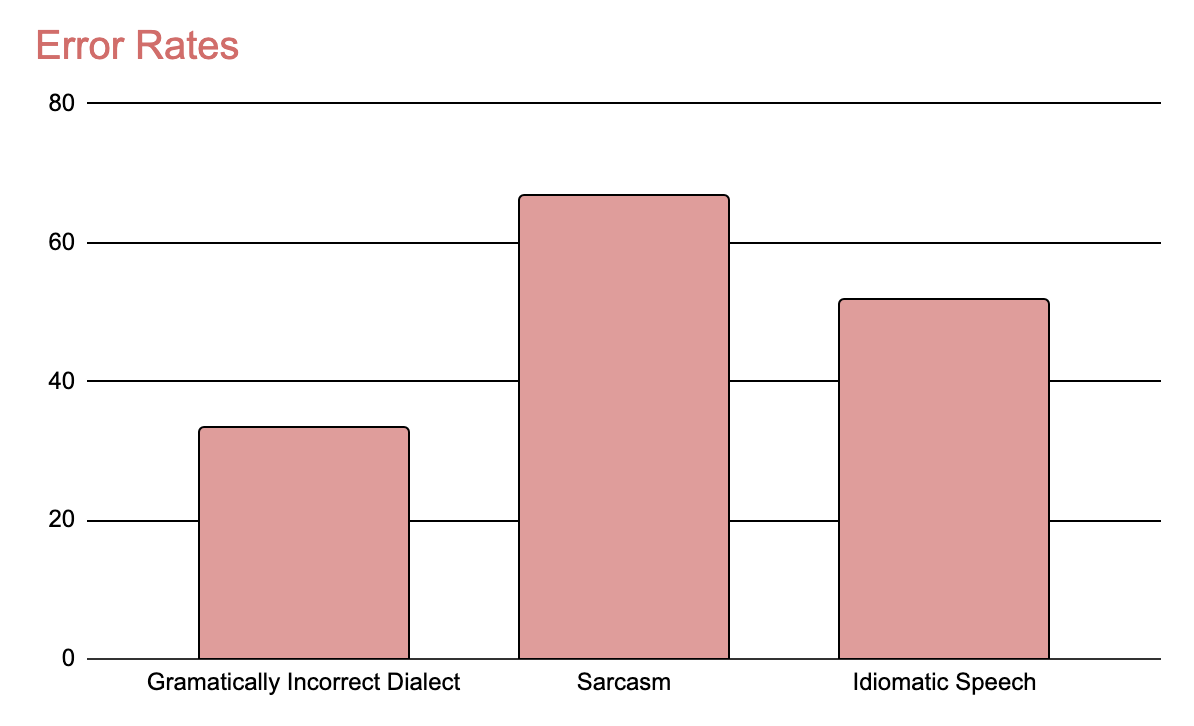
\includegraphics[width=0.7\textwidth]{figures/error_rates.png}
	\caption{prediction error rates $\in [0, 100]$ for each category of tricky example}
\end{figure}

Using a confusion matrix, we can more deeply understand what kind of misclassifications the model is making. We can see from the data that the model has a very
difficult time classifying examples where the true label is contradiction (2), as compared to those with a true label of entailment (0) or neutral (1). This is expected, because many of our tricky examples
are designed to seem like entailments, when in reality they are contradictions. Figures 2 and 3 shows the confusion
matrices on our tricky dataset and the SNLI dataset for an untuned ELECTRA-SMALL model. When we evaluated the ELECTRA-SMALL
model on the SNLI dataset it achieved an accuracy of 85.8\%.

\begin{figure}[!h]
	\centering
	\begin{minipage}{0.45\textwidth}
		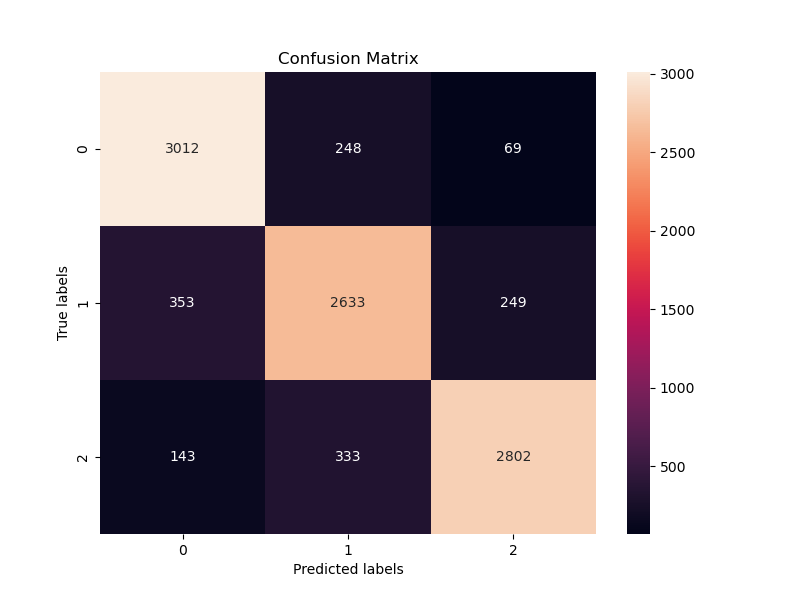
\includegraphics[width=\linewidth]{figures/snli_trained_confusion.png}
		\caption{SNLI dataset before fine tuning. lighter regions are better. notice that a clear diagonal emerges.}
	\end{minipage}
	\hfill
	\begin{minipage}{0.45\textwidth}
		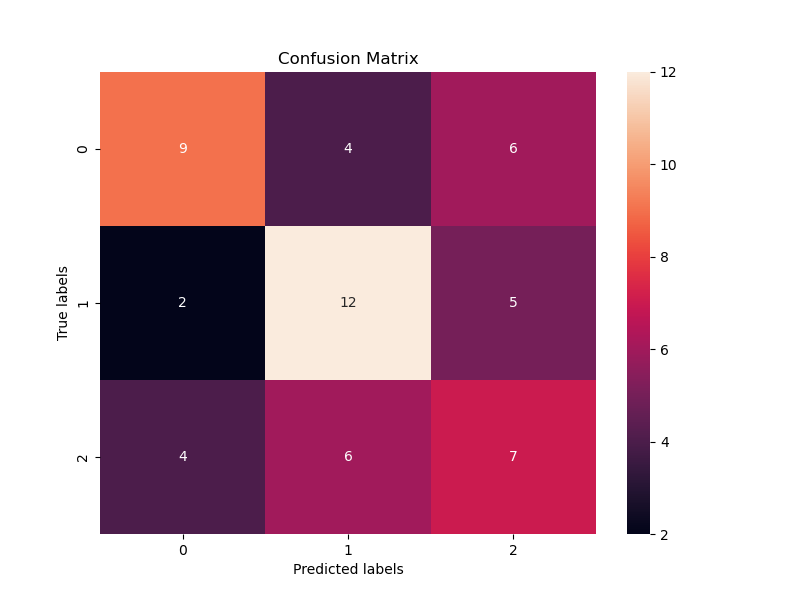
\includegraphics[width=\linewidth]{figures/tricky_trained_confusion.png}
		\caption{our tricky dataset before fine tuning. lighter regions are better.}
	\end{minipage}
\end{figure}

\section{Tuning on Adversarial Examples}
To increase the model's resilience against tricky examples, we fine tune the model on a training portion of our
tricky example dataset. The dataset is comprised of 60 hypotheses for each of the three categories discussed earlier (sarcasm,
grammatically incorrect dialect, and idiomatic speech). Each hypothesis is paired with three premises where one is an entailment,
one is neutral, and one is a contradiction. This results in a total of 180 examples. These 180 are then split into a training
portion and an evaluation portion. The train/eval split was roughly 70/30 resulting in 125 training examples and 55 evaluation
examples. The seed used to randomly split examples was 123. After fine tuning the model on our examples, the accuracy
achieved improved to 60.0\% on the “tricky examples”, up from 50.9\%. The confusion matrices for our tricky dataset before and
after fine tuning are shown in Figures 4 and 5 respectively.

\begin{figure}[!h]
	\centering
	\begin{minipage}{0.45\textwidth}
		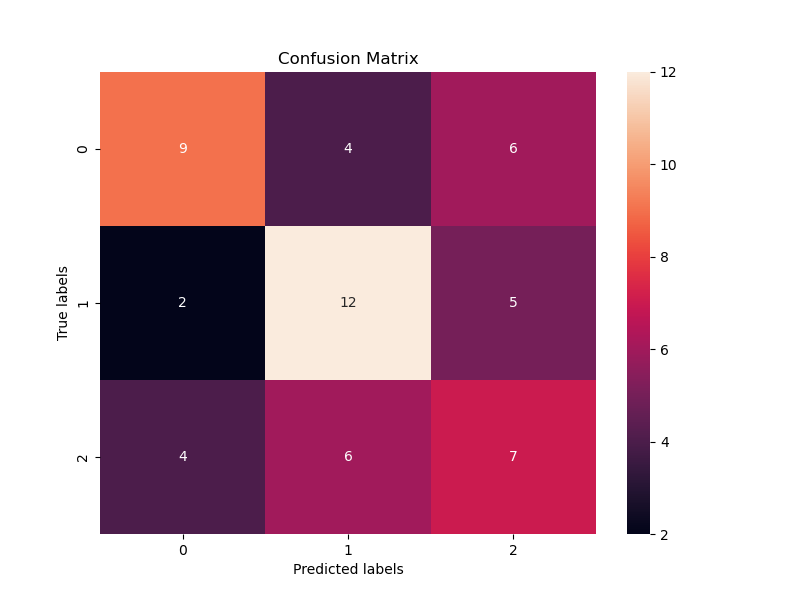
\includegraphics[width=\linewidth]{figures/tricky_trained_confusion.png}
		\caption{our tricky dataset before fine tuning. lighter regions are better. note this figure is identical to Figure 3.}
	\end{minipage}
	\hfill
	\begin{minipage}{0.45\textwidth}
		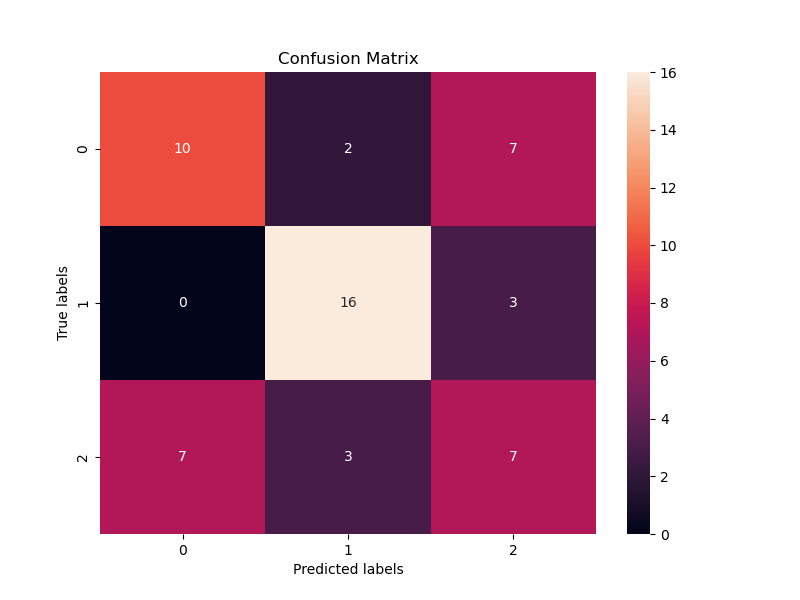
\includegraphics[width=\linewidth]{figures/tricky_tuned_confusion.png}
		\caption{our tricky dataset after fine tuning. lighter regions are better. note the emergence of a diagonal as in Figure 2.}
	\end{minipage}
\end{figure}

When re-evaluating the tuned model on the SNLI dataset, the model still achieved commensurate performance as the untuned model.
Only a small decrease in accuracy from 85.8\% to 84.6\% was observed. This drop in accuracy is expected behavior since we fine
tuned the model on examples that were significantly different from the original SNLI examples. The authors expect that
given a larger curated dataset of tricky examples, the trends we observed would continue. The models ability to accurately
pick up sarcasm, dialect, and idioms would continue to improve, while its ability to perform the original SNLI task would
continue to degrade as the fine tuning dataset increases in size. At some point, the fine tuning dataset would become
large enough as to induce catastrophic forgetting, where the model will begin to unlearn the patterns of the original
dataset altogether and start to overfit to sarcastic, dialectic, and idiomatic speech. The confusion matrices for the
untuned model and the tuned model on the original SNLI dataset are shown in Figures 6 and 7 respectively.

\begin{figure}[!h]
	\centering
	\begin{minipage}{0.44\textwidth}
		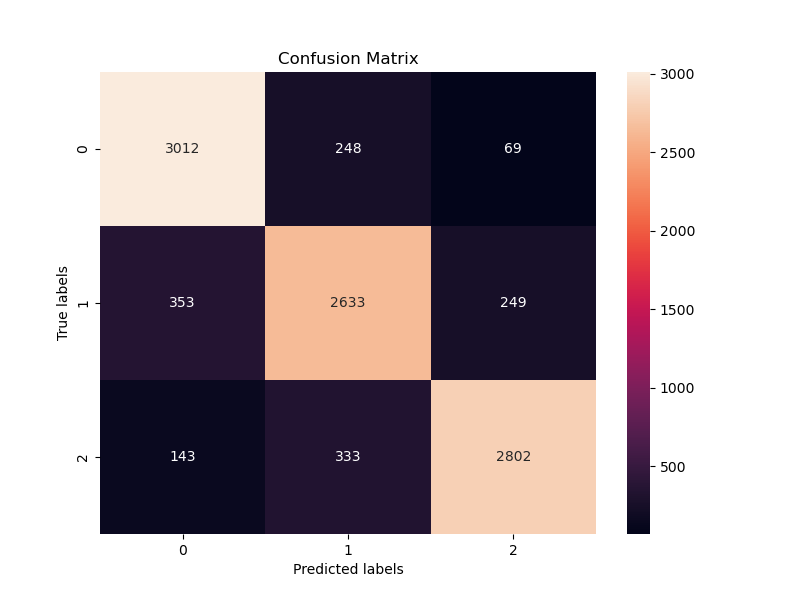
\includegraphics[width=\linewidth]{figures/snli_trained_confusion.png}
		\caption{SNLI dataset before fine tuning. lighter regions are better. note that this is identical to Figure 2.}
	\end{minipage}
	\hfill
	\begin{minipage}{0.44\textwidth}
		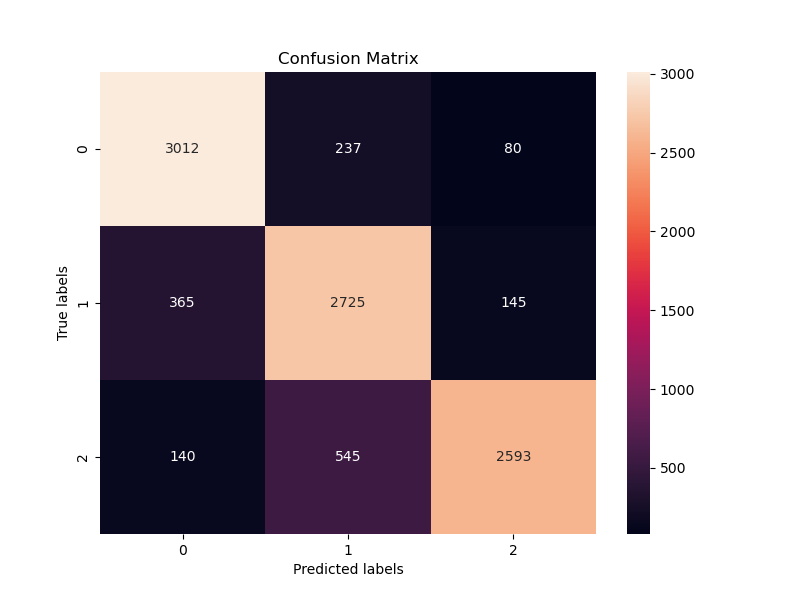
\includegraphics[width=\linewidth]{figures/snli_tuned_confusion.png}
		\caption{SNLI dataset after fine tuning. lighter regions are better.}
	\end{minipage}
\end{figure}

\newpage
We also report the accuracy, precision, recall, and f1 scores for each of our treatments. All treatments achieve tight
clusters overall with each metric being within 1\% of each other. This suggests that fine tuning on the tricky examples
improves the models general ability to correctly classify tricky examples, rather than only improving precision or recall
alone. Figure 8 provides a table of these metrics.

\begin{figure}[!h]
	\centering
	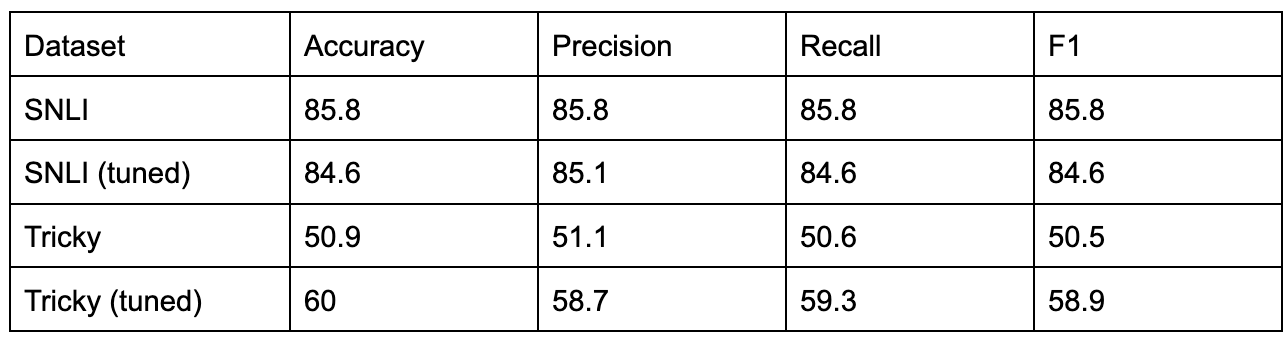
\includegraphics[width=\linewidth]{figures/nlp_final_project_metrics.png}
	\caption{reported metrics for each model-dataset treatment.}
\end{figure}

\section{Conclusion}

This work strengthens existing evidence for methods that effectively enhance the performance of NLP models in processing
complex language structures. Namely, we show the effectiveness of including adversarial examples in a fine tuning dataset
on the NLI modeling task. We demonstrate that fine tuning a model with a thoughtfully selected set of hand-annotated examples
specifically designed to challenge the model can lead to a more resilient, robust model. We also note that there is
a trade-off point when fine tuning, and that it is critical to use caution to avoid catastrophic forgetting. Specifically
consideration of the number and the nature of examples used is needed. This approach underscores the potential of targeted
tuning as a powerful tool in refining state-of-the-art models.

\bibliographystyle{plain}
\bibliography{references}

\end{document}
